\section{Vector Spaces}

\begin{dfn}
\label{dfn:vec-spa}
Let $F$ be a field. A \emph{vector space} over $F$ is a set $V$ together with two binary operations $+ : V \times V \rightarrow V$ and $\cdot : F \times V \rightarrow V$ and an element $0 \in V$ which satisfy the following properties.
\begin{enumerate*}
\item[(X)] $(V,+,0)$ is an abelian group. That is,
\begin{enumerate*}
\item[(X.1)] For all $u,v,w \in V$, we have $(u+v)+w = u+(v+w)$. \label{dfn:vec-spa:add-assoc}
\item[(X.2)] For all $v \in V$, we have $v+0 = 0+v = v$. \label{dfn:vec-spa:add-ident}
\item[(X.3)] For each $v \in V$, there is an element $-v \in V$ such that $v + (-v) = (-v) + v = 0$.
\item[(X.4)] For all $u,v \in V$, we have $u+v = v+u$.
\end{enumerate*}
\item[(Y)] $V$ is a unital $F$-module. That is,
\begin{enumerate*}
\item[(Y.1)] For all $\alpha,\beta \in F$ and $v \in V$, we have $(\alpha+\beta) \cdot v = (\alpha \cdot v) + (\beta \cdot v)$.
\item[(Y.2)] For all $\alpha,\beta \in F$ and $v \in V$, we have $(\alpha\beta) \cdot v = \alpha \cdot (\beta \cdot v)$.
\item[(Y.3)] For all $\alpha \in F$ and $u,v \in V$, we have $\alpha \cdot (v + u) = (\alpha \cdot v) + (\alpha \cdot u)$.
\item[(Y.4)] For all $v \in V$, we have $1 \cdot v = v$.
\end{enumerate*}
\end{enumerate*}
\end{dfn}

The $+$ operation is called \emph{addition} and the $\cdot$ called \emph{scalar multiplication}. We must take care not to confuse the addition and scalar multiplication on $V$ with the addition and multiplication on $F$; to help avoid confusion, we will adopt the convention that field elements are written using Greek letters ($\alpha$, $\beta$, $\gamma$) while vector space elements are written using Roman letters ($u$, $v$, $w$). As with the operations on a ring, we use a few conventions to simplify our notation. The scalar multiplication will typically be denoted by juxtaposition, and takes precedence over addition. Note also that we will use the same symbol $0$ to denote the zero in a vector space and in a field; in practice this does not lead to confusion, but where it is important to maintain the distinction we will write $0_V$ or $0_F$ to do so.

\begin{prp}
\label{prp:vec-spa:uniq}
Let $V$ be an $F$-vector space. Then zero and negatives are unique in the following sense.
\begin{enumerate*}
\item{\label{prp:vec-spa:uniq:zero}} 
If $z \in V$ such that $v+z=v$ for some $v \in V$, then $z = 0$.
\item{\label{prp:vec-spa:uniq:neg}} 
If $v,w \in V$ such that $v+w=w+v=0$, then $w = -v$.
\end{enumerate*}
\end{prp}

\begin{theproof}
Exercise.
\end{theproof}

\begin{prp}
\label{prp:vec-spa:bookkeeping}
If $V$ is an $F$-vector space, then for all $u,v,w \in V$ we have the following.
\begin{enumerate*}
\item If $u+v = u+w$, then $v = w$.
\item $0_F \cdot v = 0_V$.
\item $-(-v) = v$.
\item $(-1)v = -v$.
\item $-0_V = 0_V$.
\end{enumerate*}
\end{prp}

\begin{theproof}
Exercise.
\end{theproof}

\subsection*{Linear Transformations}

\begin{dfn}
Let $V$ and $W$ be vector spaces over a field $F$. A mapping $\varphi : V \rightarrow W$ is said to be an \emph{$F$-linear transformation} or $F$-vector space homomorphism or simply linear transformation if for all $v,w \in V$ and $\alpha \in F$ we have $\varphi(v+w) = \varphi(v) + \varphi(w)$ and $\varphi(\alpha v) = \alpha\varphi(v)$. The set of all $F$-linear transformations $V \rightarrow W$ is denoted $\Hom{F}{V}{W}$. A linear transformation $V \rightarrow V$ is called an \emph{endomorphism}, and we write $\End[F]{V}$ rather than $\Hom{F}{V}{V}$.
\end{dfn}

To every linear transformation we associate two subsets, the kernel and the image.

\begin{dfn}
Given a linear transformation $\varphi : V \rightarrow W$, the \emph{kernel} of $\varphi$ is the set $\Ker*{\varphi} = \{v \in V \mid \varphi(v) = 0\}$ and the \emph{image} of $\varphi$ is the set $\Im*{\varphi} = \{w \in W \mid \varphi(v) = w\ \mathrm{for\ some}\ v \in V\}$.
\end{dfn}

Note that, since $\varphi(0) = 0$, neither $\Ker*{\varphi}$ nor $\Im*{\varphi}$ are nonempty. In addition, by the following result we can think of $\Ker*{\varphi}$ are measuring how badly $\varphi$ fails to be injective.

\begin{prp}
Let $\varphi$ be a linear transformation. Then $\varphi$ is injective if and only if $\Ker*{\varphi} = 0$.
\end{prp}

\begin{theproof}
Suppose $\varphi$ is injective. If $v \in \Ker*{\varphi}$, then $\varphi(v) = 0$; since we also have $\varphi(0) = 0$, in fact $v = 0$. Thus $\Ker*{\varphi} = 0$. Conversely, suppose $\Ker*{\varphi} = 0$ and that $v$ and $w$ are in the domain of $\varphi$ such that $\varphi(v) = \varphi(w)$. Then $\varphi(v-w) = 0$, and since $\Ker*{\varphi} = 0$, in fact $v-w = 0$, so that $v = w$ as needed.
\end{theproof}

\subsection*{The Free Vector Space on a Set}

Given a set $X$ and a field $F$, is there an $F$-vector space which contains $X$? In the remainder of this section we will construct such a vector space $\FreeVS{F}{X}$, which we will call the free vector space on $X$. This will give us a large class of examples of vector spaces. But more importantly, these vector spaces have a nice lifting property with respect to linear transformations: if $W$ is a vector space, then every function $X \rightarrow W$ lifts uniquely to a linear transformation $\FreeVS{F}{X} \rightarrow W$.

Let $F$ be a field and $X$ a set. A function $\mu : X \rightarrow F$ is said to have \emph{finite support} if the set $\supp*{\mu} = \{x \in X \mid \mu(x) \neq 0\}$ is finite. For example, if we define $0 : X \rightarrow F$ by $0(x) = 0$ for all $x$ then $\supp*{0} = \emptyset$ is finite. Given $x \in X$, if we define $e_x : X \rightarrow F$ by $e_x(y) = 1$ if $y = x$ and $0$ otherwise, then $\supp*{e_x} = \{x\}$ is finite. The set of all functions $X \rightarrow F$ having finite support is denoted $\FreeVS{F}{X}$. Given functions $\mu,\eta : X \rightarrow F$ and $\alpha \in F$, we define $\mu+\eta,\alpha\mu : X \rightarrow F$ pointwise by $(\mu+\eta)(x) = \mu(x) + \eta(x)$ and $(\alpha\mu)(x) = \alpha\mu(x)$.

\begin{claim}
If $\mu$ and $\eta$ have finite support, then so do $\mu+\eta$ and $\alpha\mu$.
\end{claim}
\begin{theproof}
Suppose $x \in \supp{\mu+\eta}$, so that $\mu(x) + \eta(x) \neq 0$. Now either $\mu(x) \neq 0$ or $\eta(x) \neq 0$, since otherwise $\mu(x) + \eta(x) = 0$. So we have $x \in \supp*{\mu} \cup \supp*{\eta}$. Thus $\supp{\mu+\eta} \subseteq \supp*{\mu} \cup \supp*{\eta}$ is finite. Now if $\alpha = 0$, then $\supp*{\alpha\mu} = \supp*{\mu} = \emptyset$ is finite. If $\alpha \neq 0$, and if $x \in \supp*{\alpha\mu}$, then $\alpha\mu(x) \neq 0$. Dividing by $\alpha$, we have that $\mu(x) \neq 0$, so that $x \in \supp*{\mu}$. Thus $\supp*{\alpha\mu} \subseteq \supp*{\mu}$ is finite.
\end{theproof}

So this $+$ is a binary operation on $\FreeVS{F}{X}$, and this $\cdot$ is an $F$-scalar multiplication on $\FreeVS{F}{X}$.

\begin{prp}
$(\FreeVS{F}{X},+,\cdot,0)$ is an $F$-vector space, called the vector space of finitely supported functions on $X$.
\end{prp}

\begin{theproof}
Let $\mu,\eta,\chi \in \FreeVS{F}{X}$ and $\alpha,\beta \in F$, and let $x \in X$.
\begin{inparaenum}
\item[(X.1)] We have $((\mu+\eta)+\chi)(x) = (\mu+\eta)(x) + \chi(x) = (\mu(x) + \eta(x)) + \chi(x) = \mu(x) + (\eta(x) + \chi(x)) = \mu(x) + (\eta+\chi)(x) = (\mu + (\eta+\chi))(x)$. So $(\mu+\eta)+\chi = \mu+(\eta+\chi)$.
\item[(X.2)] We have $(\mu+0)(x) = \mu(x) + 0(x) = \mu(x) + 0 = \mu(x)$, so that $\mu+0 = 0$. Similarly, $0+\mu = \mu$.
\item[(X.3)] Define $-\mu : X \rightarrow F$ by $(-\mu)(x) = -\mu(x)$. Clearly $\supp{-\mu} = \supp*{\mu}$ is finite. Now $(\mu+(-\mu))(x) = \mu(x) + (-\mu)(x) = \mu(x) - \mu(x) = 0 = 0(x)$, so that $\mu+(-\mu) = 0$. Similarly, $(-\mu) + \mu = 0$.
\item[(X.4)] We have $(\mu+\eta)(x) = \mu(x) + \eta(x) = \eta(x) + \mu(x) = (\eta+\mu)(x)$. Thus $\mu+\eta = \eta + \mu$.
\item[(Y.1)] We have $((\alpha+\beta)\mu)(x) = (\alpha+\beta)\mu(x) = \alpha\mu(x) + \beta\mu(x) = (\alpha\mu)(x) + (\beta\mu)(x) = (\alpha\mu + \beta\mu)(x)$. Thus $(\alpha+\beta)\mu = \alpha\mu+\beta\mu$.
\item[(Y.2)] We have $((\alpha\beta)\mu)(x) = (\alpha\beta)\mu(x) = \alpha(\beta\mu(x)) = \alpha((\beta\mu)(x) = (\alpha(\beta\mu))(x)$, so $(\alpha\beta)\mu = \alpha(\beta\mu)$.
\item[(Y.3)] We have $(\alpha(\mu+\eta))(x) = \alpha((\mu+\eta)(x)) = \alpha(\mu(x) + \eta(x)) = \alpha\mu(x) + \alpha\eta(x) = (\alpha\mu)(x) + (\alpha\eta)(x) = (\alpha\mu+\alpha\eta)(x)$. So $\alpha(\mu+\eta) = \alpha\mu+\alpha\eta$.
\item[(Y.4)] We have $(1\mu)(x) = 1\mu(x) = \mu(x)$, so that $1\mu = \mu$.
\end{inparaenum}
\end{theproof}

\begin{claim}
If $\mu \in \FreeVS{F}{X}$, then $\mu = \sum_{x \in \supp*{\mu}} \mu(x) e_x$.
\end{claim}
\begin{theproof}
If $y \in X$, then $(\sum_{x \in \supp*{\mu}} \mu(x) e_x)(y) = \sum_{x \in \supp*{\mu}} \mu(x)e_x(y)$. Now if $y$ is not in the support of $\mu$, then this sum is precisely $0 = \mu(y)$. If $y$ is in the support of $\mu$, then every summand is 0 except for one - the $y$th term - which is equal to $\mu(y)$.
\end{theproof}

\begin{dfn}
A vector space $V$ is said to be \emph{free} on the set $X \subseteq V$ if every mapping $f : X \rightarrow W$, where $W$ is a vector space, lifts uniquely to a linear transformation $\varphi : V \rightarrow W$. That is, given $f$, there is a unique $\varphi$ such that the following diagram commutes.
\begin{center}
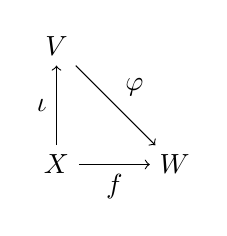
\begin{tikzpicture}[scale=0.3]
  \node (X) at (0,0) {$X$};
  \node (V) at (0,5) {$V$};
  \node (W) at (5,0) {$W$};
  \draw[->] (X) edge node [left] {$\iota$} (V);
  \draw[->] (V) edge node [above right] {$\varphi$} (W);
  \draw[->] (X) edge node [below] {$f$} (W);
\end{tikzpicture}
\end{center}
\end{dfn}

\begin{prp}
$\FreeVS{F}{X}$ is free on $X$, where we identify $x \in X$ with the element $e_x \in \FreeVS{F}{X}$.
\end{prp}

\begin{theproof}
We define $\varphi : \FreeVS{F}{X} \rightarrow W$ by $\varphi(\mu) = \sum_{x \in \supp*{\mu}} \mu(x) f(x)$. First we show that $\varphi$ is a linear transformation. Note that if $Z \subseteq X$ is finite, then \[ \sum_{x \in Z} \mu(x)f(x) = \sum_{\mathclap{\substack{x \in \supp*{\mu} \\ x \in Z}}} \mu(x)f(x) + \sum_{\mathclap{\substack{x \notin \supp*{\mu} \\ x \in Z}}} \mu(x)f(x) = \sum_{\mathclap{\substack{x \in \supp*{\mu} \\ x \in Z}}} \mu(x)f(x). \] Now 
\begin{eqnarray*}
\varphi(\mu+\eta) & = & \quad \sum_{\mathclap{x \in \supp{\mu+\eta}}} (\mu+\eta)(x)f(x) \\
 & = & \quad \sum_{\mathclap{x \in \supp{\mu+\eta}}} \mu(x)f(x) \quad + \quad \sum_{\mathclap{x \in \supp{\mu+\eta}}} \eta(x)f(x) \\
 & = & \quad \sum_{\mathclap{\substack{x \in \supp*{\mu} \\ (\mu+\eta)(x) \neq 0}}} \mu(x)f(x) \quad + \quad \sum_{\mathclap{\substack{x \in \supp*{\eta} \\ (\mu+\eta)(x) \neq 0}}} \eta(x)f(x) \quad + \quad 0 \\
 & = & \quad \sum_{\mathclap{\substack{x \in \supp*{\mu} \\ (\mu+\eta)(x) \neq 0}}} \mu(x)f(x) \quad + \quad \sum_{\mathclap{\substack{x \in \supp*{\eta} \\ (\mu+\eta)(x) \neq 0}}} \eta(x)f(x) \quad + \quad \sum_{\mathclap{\substack{x \in \supp*{\mu} \cup \supp*{\eta} \\ (\mu+\eta)(x) = 0}}} (\mu+\eta)(x)f(x) \\ 
 & = & \quad \sum_{\mathclap{\substack{x \in \supp*{\mu} \\ (\mu+\eta)(x) \neq 0}}} \mu(x)f(x) \quad + \quad \sum_{\mathclap{\substack{x \in \supp*{\eta} \\ (\mu+\eta)(x) \neq 0}}} \eta(x)f(x) \quad + \quad \sum_{\mathclap{\substack{x \in \supp*{\mu} \cup \supp*{\eta} \\ (\mu+\eta)(x) = 0}}} \mu(x)f(x) \quad + \quad \sum_{\mathclap{\substack{x \in \supp*\mu \cup \supp*{\eta} \\ (\mu+\eta)(x) = 0}}} \eta(x)f(x) \\
 & = & \quad \sum_{\mathclap{\substack{x \in \supp*{\mu} \\ (\mu+\eta)(x) \neq 0}}} \mu(x)f(x) \quad + \quad \sum_{\mathclap{\substack{x \in \supp*{\eta} \\ (\mu+\eta)(x) \neq 0}}} \eta(x)f(x) \quad + \quad \sum_{\mathclap{\substack{x \in \supp*{\mu} \\ (\mu+\eta)(x) = 0}}} \mu(x)f(x) \quad + \quad \sum_{\mathclap{\substack{x \in \supp*{\eta} \\ (\mu+\eta)(x) = 0}}} \eta(x)f(x) \\
 & = & \quad \sum_{\mathclap{x \in \supp*{\mu}}} \mu(x)f(x) \quad + \quad \sum_{\mathclap{x \in \supp*{\eta}}} \eta(x)f(x) \\ 
 & = & \varphi(\mu) + \varphi(\eta)
\end{eqnarray*}
as needed, and likewise \[ \varphi(\alpha\mu) = \sum_{\mathclap{x \in \supp*{\alpha\mu}}} (\alpha\mu)(x)f(x) = \alpha \sum_{\mathclap{x \in \supp*{\mu}}} \mu(x)f(x) = \alpha\varphi(\mu) \] since $\supp*{\alpha\mu} = \supp*{\mu}$. So $\varphi$ is a linear transformation. We also have $\varphi(e_x) = \sum_{y \in \supp*{e_x}} e_y(x)f(y) = e_x(x)f(x) = f(x)$. If $\psi : \FreeVS{F}{X} \rightarrow W$ is another linear transformation with this property, then in fact $\psi(\mu) = \psi(\sum_{x \in \supp*{\mu}} \mu(x)e_x) = \sum_{x \in \supp*{\mu}} \mu(x) \psi(e_x) = \sum_{x \in \supp*{\mu}} \mu(x) f(x) = \varphi(\mu)$ for all $\mu$, so that $\psi = \varphi$.
\end{theproof}

The proof of the lifting property of $\FreeVS{F}{X}$ is a little tedious, but once verified this property is quite strong.

\NowForSomeExercises

\begin{exercises}
\item Let $V$ be an $F$-vector space. We can define an addition operation on $\End{F}{V}$ \emph{pointwise} by $(\varphi+\psi)(v) = \varphi(v) + \psi(v)$. Show that $\End{F}{V}$ is a ring with respect to pointwise addition and composition.
\PauseExercises
\end{exercises}

\subsubsection*{Examples of Vector Spaces}

\begin{exercises}
\ResumeExercises
\item{\label{exr:hom-is-vec-spa}}
Let $V$ and $W$ be $F$-vector spaces. We can define pointwise addition and scalar multiplication operations on $\Hom{F}{V}{W}$ by $(\varphi+\psi)(v) = \varphi(v) + \psi(v)$ and $(\alpha\varphi)(v) = \alpha \varphi(v)$. Show that $\Hom{F}{V}{W}$ is an $F$-vector space with respect to these operations.

\item{\label{exr:field-ext-is-vec-spa}}
Suppose $E$ is a field and that $F \subseteq E$ is a subset which is a field under the restricted operations on $E$. (In this case we say that $E$ is an \emph{extension} of $F$.) Show that $E$ is an $F$-vector space.

\item{\label{exr:mat-is-vec-spa}}
Let $F$ be a field and let $n$ and $m$ be positive integers. Show that $\mathsf{Mat}_{n \times m}(F)$ is an $F$-vector space with respect to matrix addition and the scalar multiplication $(\alpha M)_{i,j} = \alpha M_{i,j}$.

\PauseExercises
\end{exercises}

\subsubsection*{The Free Vector Space on a Set, Part I}

\begin{exercises}
\ResumeExercises
\item
Let $X = \intrange{1}{n}$, and define $f : X \rightarrow \Mat{n}{1}{F}$ by $f(i)_{j,1} = \delta_{i,j}$ (where $\delta$ is the Kronecker delta). Show that the lift $\varphi : F_X \rightarrow \Mat{n}{1}{F}$ is bijective.

\item
Let $f : X \rightarrow Y$ be a set map. By the previous exercise, the map $e_\ast \circ f : X \rightarrow F_Y$ lifts to a unique linear transformation $F_X \rightarrow F_Y$, which we denote $F_f$ as shown in the following diagram.
\begin{center}
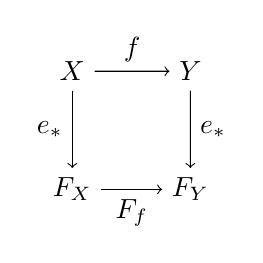
\begin{tikzpicture}[scale=0.3]
  \node (X) at (0,5) {$X$};
  \node (Y) at (5,5) {$Y$};
  \node (FX) at (0,0) {$F_X$};
  \node (FY) at (5,0) {$F_Y$};
  \draw[->] (X) edge node [above] {$f$} (Y);
  \draw[->] (FX) edge node [below] {$F_f$} (FY);
  \draw[->] (X) edge node [left] {$e_\ast$} (FX);
  \draw[->] (Y) edge node [right] {$e_\ast$} (FY);
\end{tikzpicture}
\end{center}
Show the following.
\begin{enumerate*}
\item If $f$ is injective, then $F_f$ is injective.
\item If $f$ is surjective, then $F_f$ is surjective.
\end{enumerate*}

\PauseExercises
\end{exercises}

We will denote an element $\mu \in F_X$ as a \emph{formal sum} $\mu = \sum_{x \in X} \mu_x e_x$.

\subsubsection*{Linear Transformations and Isomorphisms}

\begin{exercises}
\ResumeExercises
\item Show the following.
\begin{enumerate*}
\item The identity map $1 : V \rightarrow V$ is a linear transformation.
\item If $\varphi$ and $\psi$ are linear transformations, then the composite $\psi\varphi$ is as well (if it exists).
\end{enumerate*}

\item A linear transformation $\varphi : V \rightarrow W$ which is also bijective is called an \emph{isomorphism}. In this case we say that $V$ and $W$ are \emph{isomorphic}, denoted $V \cong_F W$ or just $V \cong W$. Show the following.
\begin{enumerate*}
\item $V \cong V$.
\item If $V \cong W$ then $W \cong V$.
\item If $V \cong W$ and $W \cong U$ then $V \cong U$.
\end{enumerate*}

\item Let $F$ be a field and fix a matrix $A$ of dimension $m \times n$ over $F$. Show that the mapping $\varphi : \Mat{n}{1}{F} \rightarrow \Mat{m}{1}{F}$ given by $\varphi(X) = AX$ is an $F$-linear transformation.
\end{exercises}